\section{Drehstrom- Asynchronmaschinen (DAM)}
    \subsection{Aufbau der DAM}
        \begin{tabular}[c]{| p{3cm} | p{5cm} | p{4cm} | p{5cm} |}
            \hline
            Name &
            Aufbau &
            Positiv &
            Negativ \\
            \hline
            Schleifringläufer &
            Ständerwicklung und Läuferwicklung sind für Drehfelder gewickelt. Die Läuferwicklunganschlüsse sind rausgezogen, um einem Widerstand einzuschliessen. &
            Mit deiesem Widerstand lässt sich die Drehzahl regulieren &
            Die Schleifkontakte reduzieren den Wirkungsrad und erhöhen den Verschleiss. \\
            \hline
            Kurzschlussläufer / Käfigläufer &
            Die Läuferwicklungen sind immer kurzgeschlossen. &
            Es kann ein beinahge reibungsloser und verschleisfreier Betrieb ermöglicht werden &
            Die Drehzahl ist beinahe die Drehfeldfrequenz durch die Polzahl \\
            \hline
        \end{tabular}
    \subsection{Funktionsprizip}
        Das vom Ständer erzeugter Drehfeld erzeugt im stillstehenden, kurzgeschlossenen Läufer einen Drehstrom. Der Schlupf ist bei einem stillstehendem Läufer 1. Dieser Drehstrom erzeugt im Läufer ein Drehmoment. Dieses Drehmoment beschleunigt den Läufer.Durch verringert sich Schlupf, was wiederum ein kleineres Drehmoment nachsichtzieht. Bei einem Läufergeschwindigkeit, welche gelcih schnell ist wie das Drehfeld, reslutiert eine relative Geschwindigkeit von 0 (Schlupf von 0)$\rightarrow $ kein Drehmoment. Das heisst der DAM bewegt sich immer mit möglichst kleinem Schlupf.

    \subsection{Ersatzschaltbild}
        Da der DAM nach dem Induktionsgesetz funktionniert, kann man ihn gut als Trafo- Ersatzschaltbild darstellen. Der veränderliche Wirkwiderstand (Lastwiderstand) ist die mechanische Last. Das heisst die Verlustleistung über dem Widerstand ist die Mechanische Nutzleistung (minus die Reibungsverluste). Diese ist, wie man sieht von dem Schlupf abhnängig.
        \abb{images/ersatzschaltbild_DAM}{12cm}{Ersatzschaltbild des DAM mit Last}

     
     
    \subsection{Formeln zur Asynchronmaschine}
    \begin{tabular}[c]{ | p{6cm} | p{9cm} |}
    	\hline
    	Drehfeldzahl $[s^{-1}]$ bzw $[min^{-1}]$ & $n_d=\frac{f}{p}$ bzw
    	$n_d=\frac{f\cdot 60}{p}$\\
    	\hline
    	Schlupf $[-]$ & $s=\frac{n_d-n}{n_d}$\\
    	\hline
    	Zugeführte Wirkleistung & $P_{zu}= P_{el}=3\cdot U_1 \cdot I_1 \cdot
    	\cos\varphi$\\
    	\hline
    	Drehfeldleistung & $P_\delta=P_{el}-3\cdot\left(I_1^2\cdot R_1 +
    	P_{Fe}\right)=3\cdot\frac{R_2^\prime}{s}\cdot I_2^{\prime 2}$\\
    	\hline
    	Wellenleistung ohne Reibung & $P_{mech}=P_\delta-3I_2^{\prime 2}\cdot
    	R_2^\prime=(1-s)\cdot P_\delta$\\
    	\hline
    	Läuferverlustleistung & $P_{v2}=3\cdot R_2^\prime\cdot I_2^{\prime
    	2}=s\cdot P_\delta$\\
    	\hline
    	Drehmoment & $M=\frac{P_{mech}}{2\cdot\pi\cdot
    	n}=\frac{P_\delta}{2\cdot\pi\cdot n_0}$\\
    	\hline
    	Kippmoment & $M_{kipp}=\frac{3\cdot U_I^2}{4\pi\cdot
    	n_1}\cdot\frac{1-\sigma}{R_1(1-\sigma)+\sqrt{R_1^2+X_1^2}}\approx\frac{3\cdot
    	U_1^2}{4\pi\cdot n_1 \cdot X_\sigma}$\\
    	\hline
    	Klosssche Gleichung &
    	$\frac{M}{M_k}=\frac{2}{\left(\frac{s}{s_{kipp}}+\frac{s_{kipp}}{s}\right)}=\frac{2
    	s s_k}{s^2+s_k^2} $\\
    	\hline
    	Kippmoment Dreieckschaltung& $M_k= Faktor \cdot M_N$\\
    	\hline
    	für Sternschaltung & $M_{Stern}= \frac{M_\Delta}{3}$\\
    	\hline
    \end{tabular}
    
    \subsection{Drehmomentkennlinie}
        \begin{minipage}{5cm}
            \abb{images/Drehmomentkenn_DAM.png}{5cm}{$M = f(s)$}   
        \end{minipage}
        \begin{minipage}{13cm}
            $M_K = Kippmoment = Maximales Drehmoment$ \\
            $M_K \approx \frac{3 \cdot U_1^2}{4\cdot \pi \cdot n_1 \cdot X_\sigma}$ \\
            $X_\sigma = X_{\sigma 1} + X_{\sigma 1}^`$ \\
            $\frac{M}{M_K}\approx \frac{2}{\frac{s}{s_k}+\frac{s_k}{s}}$ \\
            $s_k = \frac{R_2^`}{\sqrt{R_1^2 + X_1^2}} \approx \frac{R_2^`}{X_\sigma}$    
        \end{minipage}
        \newpage

    \subsection{Ortskurve des DAM, Heyland- Kreis}
        \begin{minipage}{9cm}
            \abb{images/Heylandkreis.png}{8cm}{Heylandkreis mit Leistungs- und Momenteneinteilung}
        \end{minipage}
        \begin{minipage}{8cm}
            \abb{images/Heylandkreis_schlupf.png}{7cm}{Heylandkreis mit Schlupfskalierung}
        \end{minipage} \\
        \begin{minipage}{10.5cm}
            \begin{enumerate}     
                \item Den Massstab für den Strom wählen zB. $m_I=\frac{0.2 A}{mm}$
                \item Den Massstab für die Leistung berechnen: $P_{gesamt}=3U_N I_{Ph}$ $m_P=3U_N m_I$
                \item Den Massstab für das Drehmoment berechnen: $M=\frac{P_\delta}{2\pi n_0};$  $m_M= \frac{p\cdot m_P}{2\pi f}$  p = Polpaar
                \item $s=0 \rightarrow s_{0}$ messen und einzeichnen
                \item $s=1 \rightarrow s_{1}$ messen und einzeichnen
                \item Verlustleistung bei $s_{0}$ herauslesen ($P_{Fe}$) (ev. wenn nicht schon getan, mit \\ $P_{FE} = U \cdot I_{Wirk}$ den Leistungs-Massstab bestimmen.)\\
                \item $\perp$ vom Mittelpunkt von $\overline{s_{0}s_{1}}$
                \item Schnittpunkt auf $s_{0}- Achse (Richtung -j) = M$
                \item Kreis um M mit Schnittpunkt $s_{0}$ und $s_{1}$
                \item $I_N =$ Tangente auf dem Kreis vom Ursprung (0,0)
                \item $P_{v1}$ bei $s_{1}$ ausrechnen = $P_{R_1}$ von der Parallele zur J-Achse, welche durch M geht nach oben abtragen.
                \item Verbindung des Punktes zu $s_{0}$ verlängern $\rightarrow$ $s_{\infty}$
                \item \textit{ Bei Vereinfachung $R_{Cu}=0:\\ s_{0}$ auf Imaginär- Achse; $s_{\infty}$ auf Imaginär-Achse}
                \item Schlupf- Skalierung: $\perp$ auf $\overline{s_{\infty}M}$
                \item Schnittpunkt mit Verlängerung $\overline{s_{1}s_{\infty}}= 1$
                \item Schnittpunkt mit $\overline{s_{0}s_{\infty}}= 0$
                \item Dazwischen lineare Unterteilung
            \end{enumerate}
        \end{minipage}
        \begin{minipage}{7cm}
            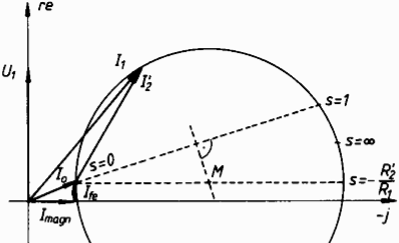
\includegraphics[width=6cm]{../ElMasch/images/StromortskurveDAM.png}\\
            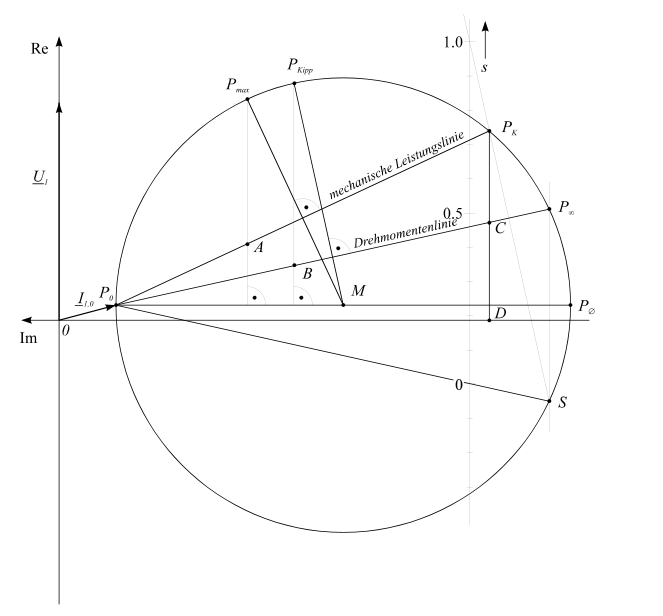
\includegraphics[width=8cm]{../ElMasch/images/OssannakreisPkipp.png}
        \end{minipage}